%!TEX root = ../template.tex
%%%%%%%%%%%%%%%%%%%%%%%%%%%%%%%%%%%%%%%%%%%%%%%%%%%%%%%%%%%%%%%%%%%%
%% chapter2.tex
%% NOVA thesis document file
%%
%% Chapter with the template manual
%%%%%%%%%%%%%%%%%%%%%%%%%%%%%%%%%%%%%%%%%%%%%%%%%%%%%%%%%%%%%%%%%%%%

\typeout{NT FILE chapter2.tex}%

\chapter{Work plan}
\label{cha:work_plan}


\section{Characterization of the solution}
\label{sec:characterization_of_the_solution}

 The IOPT-Tools environment provides robust support for modeling, verifying, and generating code for individual controller sub-models using Input-Output Place-Transition (IOPT) Petri nets \cite{iopttools, barros2004, RefiningIOPT}. However, a notable challenge arises in distributed control systems, particularly those adhering to the Globally Asynchronous, Locally Synchronous (GALS) paradigm, where decomposed sub-models require inter-communication \cite{galsactd, Barrosadd}. As identified in Section~\ref{subsec:communication_gap}, the existing automatic code generation primarily focuses on the internal logic of each sub-model, necessitating manual implementation of the communication links between them. This dissertation plan directly addresses this gap by proposing an automated code generation tool.
 
 The core objective is to develop a mechanism that analyzes decomposed IOPT sub-models and automatically generates the necessary communication infrastructure code, thereby streamlining the development of distributed control systems and automating the creation of efficient and reliable data exchange pathways.
 
 
 
  \textbf{Characterization of the Automated Communication Code Generation Tool}: This proposed tool will function as an integral extension within the IOPT-Tools environment, designed to bridge the gap between high-level IOPT model specification and the concrete implementation of inter-controller communication. Its operation can be characterized by its inputs, processing logic, and outputs:

\begin{itemize}
    \item \textbf{Input to the Tool:} The primary input to the automated code generation tool will be the decomposed IOPT Petri net sub-models themselves, as generated by IOPT-Tools' existing net splitting operation (detailed in \ref{sub:net_addicion}). Crucially, the tool will analyze the structural information inherent in these decomposed models, specifically:
    \begin{itemize}
       \item \textbf{Synchronized Transitions:} These represent the logical communication points where interactions between sub-models are required. The tool will identify these shared synchronization points across different sub-models.
        \item \textbf{Shared Places:} In some decomposition scenarios, shared places may also indicate data exchange requirements or common resources, which the tool will interpret as communication needs.
       \item \textbf{Time Domain (TD) Annotations:} For GALS systems, the tool will leverage the Time Domain attribute associated with IOPT Petri net nodes (places and transitions). Communication channels identified between transitions belonging to distinct time domains will be automatically flagged for asynchronous communication protocols, aligning with the GALS paradigm.Conversely, intra-domain communication needs will be identified for synchronous protocols.
        \item \textbf{Asynchronous Channels (ACs):} The explicit modeling of Asynchronous Channels within the IOPT-GALS framework will directly inform the tool about required communication pathways and their associated time domains.
    \end{itemize}

    \item \textbf{Automated Processing and Configuration:} Based on the analysis of the IOPT model structure, the tool will automatically:
    \begin{itemize}
        \item \textbf{Identify Communication Channels:} Determine the precise data or event exchanges required between sub-models.
        \item \textbf{Infer Communication Requirements:} Extract properties such as data size, directionality, and frequency of interaction from the IOPT model semantics.
        ]\item \textbf{Propose/Select Communication Protocols:} Guided by the characteristics of the identified communication (e.g., synchronous vs. asynchronous, point-to-point vs. bus, data rate needs as analyzed in \ref{sec:communication_support_technologies}), the tool will propose suitable communication protocols (e.g., UART for asynchronous event transfer, SPI/I2C for local synchronous data exchange , FIFO+Handshake for robust inter-domain data streaming, or UDP for lightweight networked communication).
    \end{itemize}

    \item \textbf{Output: Generated Communication Code:} The primary output of the tool will be ready-to-integrate source code in either C or VHDL. This generated code will encompass the essential communication infrastructure, including:
    \begin{itemize}
       \item \textbf{Low-level Driver Code:} Implementations of the chosen communication protocols (e.g., UART initialization, SPI master/slave logic, I2C routines, FIFO buffer management with handshake signals).
        \item \textbf{API Wrappers:} Abstraction layers that allow the core IOPT controller logic (generated by existing IOPT-Tools features) to seamlessly interact with the communication hardware without needing to manage low-level details.
        \item \textbf{Configuration Files/Headers:} Automatically generated files defining parameters such as baud rates, slave addresses, data frame formats, or buffer sizes, ensuring consistent setup across communicating sub-models.
        \item \textbf{Interface Logic for GALS Communication:} Specifically for inter-domain communication, the generated code will include synchronization mechanisms (e.g., FIFOs with handshake signals, as discussed in Section \ref{sub:fifo+handshake})] to reliably cross clock domains.
    \end{itemize}

    \item \textbf{Integration with IOPT-Tools and User Interaction:} The tool will be designed to integrate smoothly within the existing IOPT-Tools web-based environment. While the core generation will be automated, a graphical interface will allow users to:
    \begin{itemize}
        \item \textbf{Visualize Identified Channels:} Display the detected communication links between sub-models.
        \item \textbf{Review Proposed Protocols:} Show the protocols suggested by the tool.
        \item \textbf{Configure Parameters (if needed):} Provide options for users to override default protocol selections, assign specific hardware pins, or configure network addresses for advanced scenarios, thereby offering flexibility while retaining automation benefits.
        \item \textbf{Initiate Code Generation:} A clear interface to trigger the generation of communication-specific code alongside the existing controller logic.
    \end{itemize}
\end{itemize}

Figure~\ref{fig:distributed_system_example} illustrates a typical distributed control system architecture, composed of multiple micro-controllers (representing IOPT sub-models) interacting via various communication channels. This visual representation underscores the complexity and the need for automated communication management that this work addresses. Each "Micro-controller" in the figure would correspond to an independently operating IOPT sub-model, potentially residing in distinct time domains (represented conceptually by T1 and T2), and the "Communication channels" are the critical links that the proposed tool will automatically generate code for.The generated code will be designed to be implemented within the communication module of each controller (\ref{fig:representation}), ensuring seamless integration with the existing controller logic, thereby reducing development effort, minimizing manual coding errors, and enhancing the overall utility of the IOPT-Tools framework for complex distributed applications.

 
\begin{figure}[htbp]
  \centering
  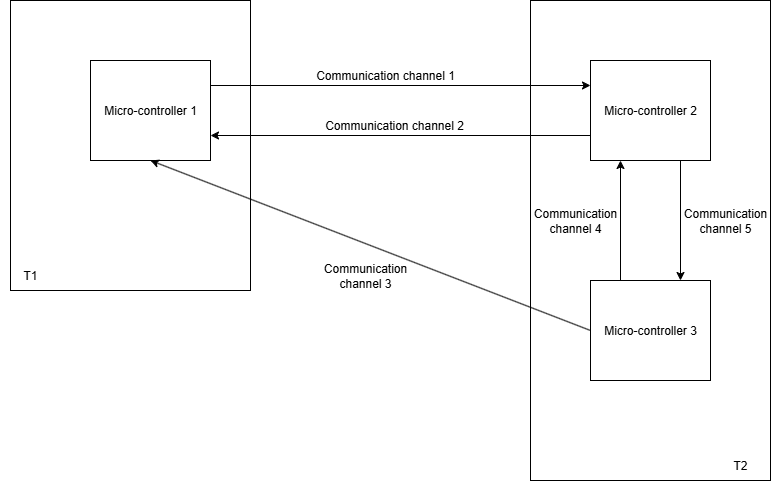
\includegraphics[width=0.8\textwidth]{solution_abstract.png}
  \caption{Example of a Distributed Control System Architecture with Communication Channels.}
  \label{fig:distributed_system_example}
\end{figure}

 \begin{figure}[htbp]
  \centering
  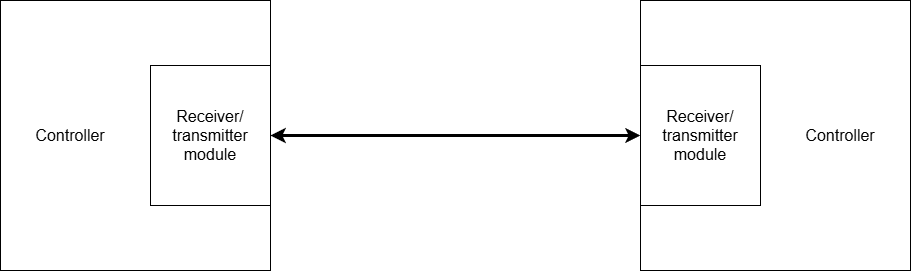
\includegraphics[width=0.6\textwidth]{Chapters/Figures/Diagrama.png}
  \caption{Solution representation.}
  \label{fig:representation}
\end{figure}
 
 
 
\section{Gantt Diagram }
\label{sec:gant_diagram}


The detailed work plan will be visualized using a Gantt diagram, which illustrates the project's timeline, task durations. This diagram, which will be provided as an figure ~\ref{fig:GanttChart}, is structured around the key tasks outlined in the following section.

 \begin{figure}[htbp]
  \centering
  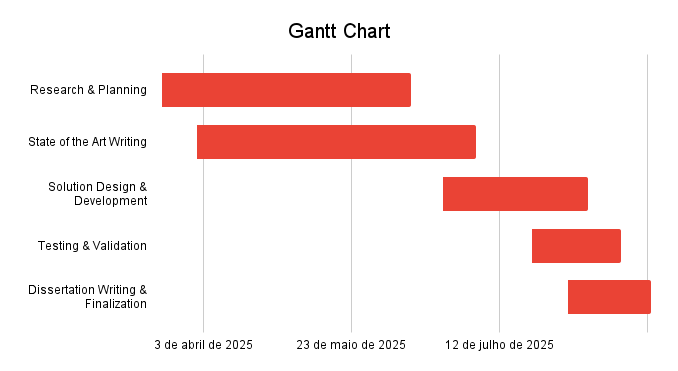
\includegraphics[width=0.8\textwidth]{Chapters/Figures/GanttChart.png}
  \caption{Project Timeline (Gantt Chart).}
  \label{fig:GanttChart}
\end{figure}
 

\section{Task Building}
\label{sec:task_building}

\begin{enumerate}
    \item \textbf{Research and Planning:} This initial phase involves comprehensive literature review, understanding the context of the problem, analyzing existing IOPT-Tools functionalities, and conceptualizing the overall design and architecture for the automated communication code generation tool.



    \item \textbf{State of the Art Writing:} Dedicated to the formal documentation of the theoretical and technological foundations underpinning the research, including in-depth discussions on Petri nets, IOPT Petri nets, GALS systems, and various communication technologies. This task heavily relies on the research conducted in the first phase.





    \item \textbf{Solution Design and Development:} 
	This core phase will be divided into several sequential steps, as detailed below:   
    
    \begin{itemize}
    \item \textbf{Technology Selection and Scenario Setup}:
	This initial stage will focus on selecting a communication technology , from the ones study at \ref{sec:communication_support_technologies}, and building the scenario with Arduinos for that tecnology, this will at least include one communication channel as described in~\ref{fig:distributed_system_example}, the initial choice of the communication technology with follow this criteria:
    \begin{itemize}
    \item Relevance to typical distributed control scenarios, especially those encountered in embedded systems and industrial automation.
    \item Availability of compatible hardware modules for Arduino platforms to ensure rapid prototyping.
    \item Simplicity of implementation and debugging, favoring protocols with strong community support and documentation.
    \end{itemize}
    \item \textbf{Development of foundational code}:  
This stage will focus on writing the necessary code to program the Arduino in the scenario chosen before, utilizing the selected communication technology to establish reliable interaction between controllers. This foundational work will serve as a baseline for subsequent automation efforts. 


    \item \textbf{Implementation of an automated code generation tool}:  
 Building upon the foundational code, this crucial step involves designing and developing the core automated code generation tool. This tool will be architected with extensibility in mind from the start, enabling it to incorporate different communication protocols identified in \ref{sec:communication_support_technologies}. Its primary function will be to automatically generate the necessary communication infrastructure code for IOPT sub-models, significantly streamlining the development process and reducing manual coding effort.
 
    \item \textbf{Integration with IOPT-Tools}:  
Once the code generation engine is functional, the next phase will consist of integrating the engine and its graphical interface into the IOPT-Tools environment. This ensures seamless interoperability and extends the toolchain functionality for users of IOPT-tools.

    \item \textbf{Extension to support additional communication technologies}:  
If time and resources permit, the developed tool's modular architecture will be leveraged to integrate support for additional communication technologies. This process will involve adapting the existing code generation framework to incorporate the specific requirements of new protocols, further enhancing its flexibility and reusability.
\end{itemize}


    \item \textbf{Testing and Validation:} Focused on ensuring the robustness and correctness of the developed solution. This includes unit testing of individual code generation modules, integration testing of the tool within IOPT-Tools, functional validation with representative distributed IOPT petri nets.
    
    
    
    
    
    
    
    

    \item \textbf{Dissertation Writing and Finalization:} This ongoing task involves the continuous process of documenting all aspects of the research, including the work plan, implementation details, results, and conclusions. It also covers the preparation of any user manuals or tutorials for the developed tool, and the final review and preparation of the entire dissertation for submission and defense.
\end{enumerate}